\documentclass[10pt,a4paper]{ctexart}
\usepackage[margin=0.82in]{geometry}
\usepackage{amsmath,booktabs,graphicx,hyperref,float}
\graphicspath{{figures/}}
\hypersetup{colorlinks=true,linkcolor=black,citecolor=blue,urlcolor=blue}
\newcommand{\um}{\ensuremath{\mu\mathrm{m}}}
\newcommand{\wn}{\ensuremath{\mathrm{cm}^{-1}}}
\title{双角度 FTIR 条件下碳化硅外延层厚度测量：\\7.4--7.6 \um\ 候选区间的证据链}
\author{蔡文傑\\厦门大学\\\href{mailto:19020232202343@stu.xmu.edu.cn}{19020232202343@stu.xmu.edu.cn}}
\date{}
\begin{document}\maketitle
\section*{摘要}
碳化硅外延层厚度是功率器件结构设计中的关键几何量。红外反射谱中的干涉条纹能够提供非接触式厚度信息，但条纹周期并不等同于已经标定的厚度：复折射率色散、多重反射、入射角和仪器响应都会影响反演。本文分析同一片 SiC 外延片在 $10^\circ$ 与 $15^\circ$ 下采集的 FTIR 反射谱。最终的主测量结论为：该样品外延层厚度目前可支持的候选区间是\textbf{7.4--7.6 \um}。在受约束的双角度传输矩阵模型中，局部最小点为 $7.465\,\um$，联合 RMSE 为 0.00171152；该数值仅是给定光学模型下的代表值，不被表述为独立认证的真值。

证据链分为四层：多种预处理与滑窗 FFT 首先确认稳定相位尺度；简化 FOD 路线显示不同折射率约定会造成明显厚度差异；带有介电函数约束的双角度 TMM 将相位映射为共享厚度；剖面扫描、分段残差自助法和频带权重扰动用于检验局部稳健性。四种权重方案的最小点仅移动 $0.020\,\um$，但 $15^\circ$ 残差更大且高度相关，外延层等离子体尺度参数触及上界。因此，本文报告的是在现有模型与数据下具有内部一致性的厚度测量结论，而不是绝对精度声明。要获得准确度和完整物理不确定度，仍需轮廓仪、截面 SEM 或椭偏仪等独立计量验证。

\noindent\textbf{关键词：} 碳化硅；外延层；傅里叶变换红外光谱；厚度测量；传输矩阵；可辨识性

\section{问题与证据标准}
SiC 外延层的厚度影响漂移区的器件设计和工艺一致性。空气--外延层、外延层--衬底两个界面的反射会在红外波段形成干涉结构，因此 FTIR 具有快速、非接触的优势。已有研究已将条纹级差和 FTIR 反射用于 SiC 外延层厚度分析\cite{Li2010,Dong2012}。然而，条纹相位同时受厚度、色散、吸收和界面对比度控制；仅凭一个条纹间距给出精确厚度，忽略了该逆问题的多解性。

本文不把一个优化器输出直接当作测量真值，而是区分四种证据：条纹是否真实存在；物理模型如何把条纹映射为厚度；结果在模型内是否稳定；以及是否有外部计量支持绝对准确度。这样的区分使数值结果的强度与其证据相匹配。

\begin{figure}[H]\centering
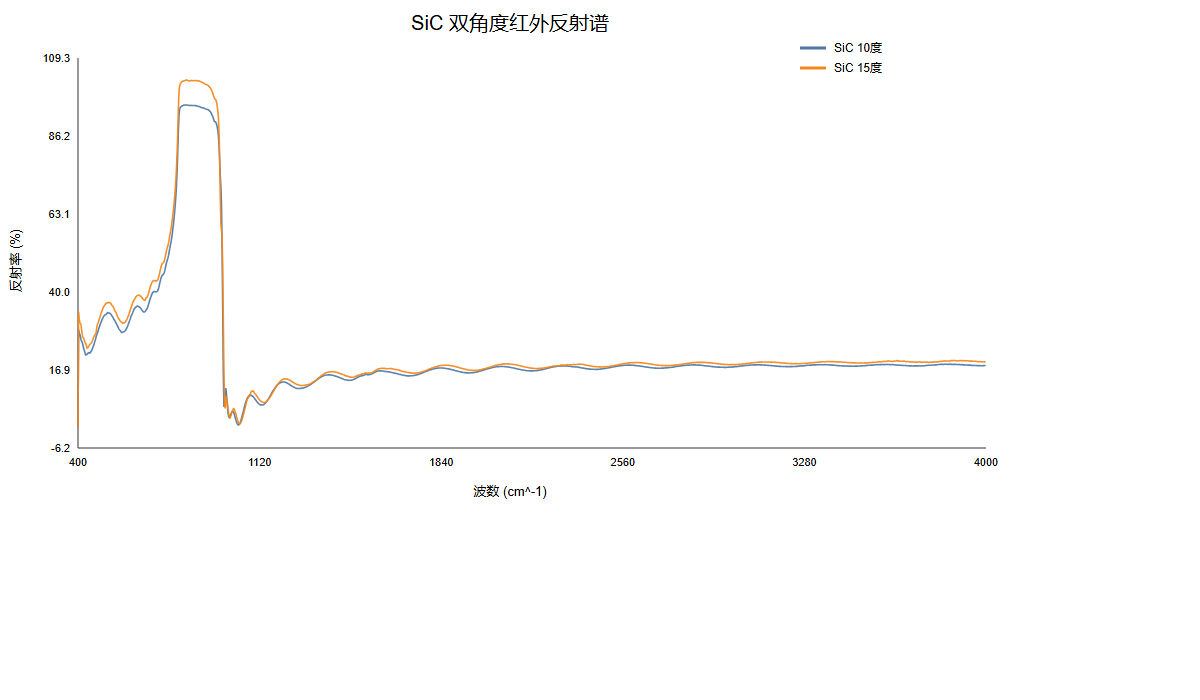
\includegraphics[width=.94\linewidth]{paper_fig00_sic_dual_angle_raw.png}
\caption{SiC 双角度原始反射谱。振荡结构构成相位反演的起点；其变化的包络与角度差异也说明不能把谱线简化为理想正弦波。}
\label{fig:raw-cn}
\end{figure}

\subsection*{符号、单位与阅读约定}
为使后续公式可直接对应数据和模型，表 \ref{tab:symbols-cn} 先固定符号。波数均以 \wn\ 计，厚度以 \um\ 计；$a$ 表示入射角索引而非拟合系数。复数折射率、残差和介电参数只在其所属模型内使用，避免把拟合自由度误读为独立测量量。
\begin{table}[H]\centering\small
\caption{本文核心符号及其物理角色。}\label{tab:symbols-cn}
\begin{tabular}{p{.18\linewidth}p{.42\linewidth}p{.26\linewidth}}\toprule
符号 & 含义 & 在何处使用\\\midrule
$\nu,\lambda_0$ & 波数与真空波长，满足 $\lambda_0=10^4/\nu$ & 所有相位与频域计算\\
$d,\theta_0,\theta_1$ & 外延层厚度、空气入射角和膜内折射角 & 干涉相位与 Snell 定律\\
$n,k,\tilde n$ & 折射率实部、消光系数与复折射率 $n+{\rm i}k$ & 色散 FOD 与 TMM\\
$\Delta\nu,\Delta m_i$ & 条纹周期与第 $i$ 个极值的级次差 & 峰距、FOD 和 FFT\\
$R_{\rm obs},R_{\rm model}$ & 观测反射率与正演模型反射率 & 拟合目标和残差\\
$\alpha_a,b_a$ & 第 $a$ 个角度的仿射尺度与偏置 & 变量投影校准\\
$\eta,\nu_p,\gamma$ & 材料参数向量、等离子体频率与 Drude 阻尼 & Dong/TMM 物理约束\\
$r_i,\rho_1,w_i$ & 残差、一阶自相关与频带权重 & 诊断与稳健性分析\\\bottomrule
\end{tabular}
\end{table}

\subsection*{测量假设、数据统一与预处理边界}
综合既有研究稿的实验叙述，本文将以下条件写成可检验的测量前提，而非无条件事实：（1）测量区域内外延层与衬底界面近似平行，故厚度可用共享标量 $d$ 表示；（2）两个角度来自同一片晶圆，因而应由同一厚度解释；（3）外延层与衬底具有足以产生可辨识干涉的光学差异；（4）FFT 与 FOD 仅负责发现相位尺度和候选盆地，TMM 才承担主反演；（5）Dong2012 参数是 4H--SiC 光学响应的约束来源，不能被误读为本样品已实测的材料参数。若任一前提不成立，后文的误差诊断将优先暴露其后果，而不是用更多自由参数掩盖它。

原始反射率以波数为横坐标。为使频域处理的采样间隔有明确含义，先按波数排序、将百分数反射率统一为小数，并插值到等间隔网格 $R_{\rm grid}(\nu_j)=\operatorname{interp}(\nu_j;\nu_{\rm raw},R_{\rm raw})$；真空波长换算为 $\lambda_0(\um)=10^4/\nu(\wn)$。中心化、移动平均、低阶多项式、滚动基线和一阶差分并行使用：它们只用于检验慢变背景移除后主周期是否仍存在，不进入最终物理模型的可调参数。

\section{数据与光学模型}
数据来自同一片 SiC 外延片在 $10^\circ$ 和 $15^\circ$ 入射角下的反射谱；每个原始工作簿含 7,469 个波数--反射率点。主分析窗口为 $1500$--$4000\,\wn$，以保留多个可见干涉周期，同时避免将低波数复杂吸收直接解释成厚度信息。项目材料未提供轮廓仪、椭偏、截面 SEM 或标准片厚度，故不能据此计算绝对误差。

多种预处理均给出约 $250\,\wn$ 的全局主周期；在宽度 $1200\,\wn$、步长 $250\,\wn$ 的滑动窗口中，主周期范围为 $244.537$--$256.000\,\wn$。图 \ref{fig:sliding-cn} 将这一结果以局部窗口展示。它加强了“干涉尺度真实存在”的判断，但并不消除折射率口径带来的厚度定标歧义。

\begin{figure}[H]\centering
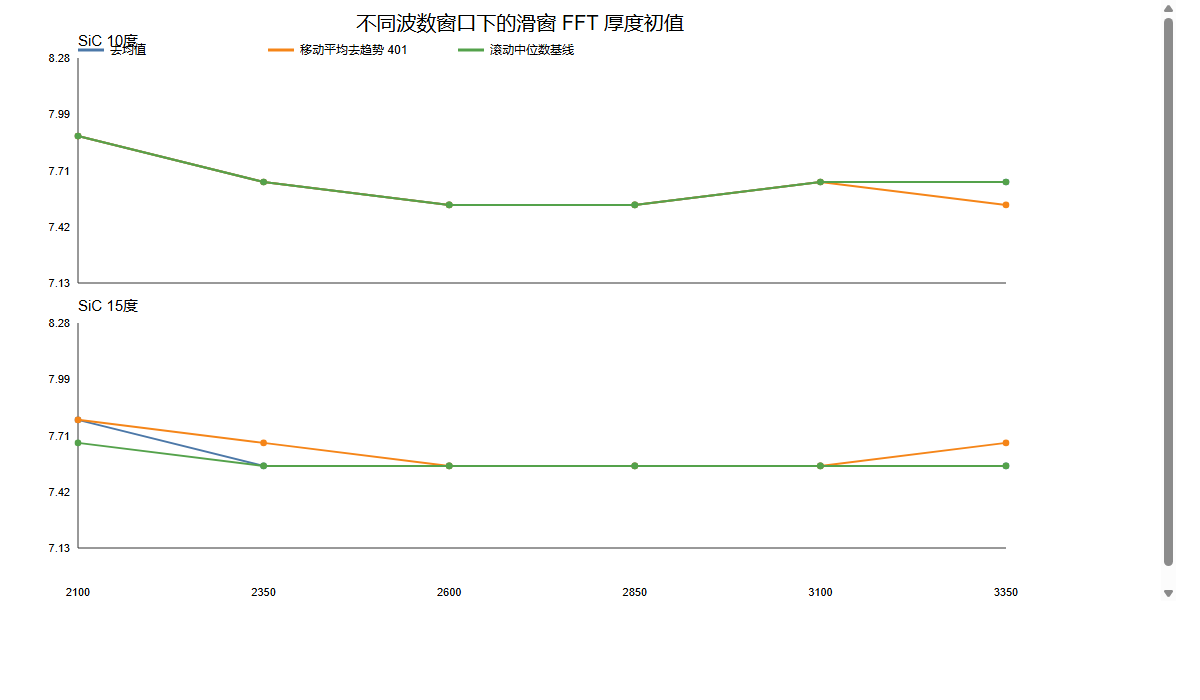
\includegraphics[width=.84\linewidth]{sliding_fft_thickness_by_window.png}
\caption{滑窗 FFT 的主周期与相应厚度种子。各窗口周期集中于约 $250\,\wn$，支持条纹尺度的局部稳定性；种子厚度仍随有效折射率约定而变。}
\label{fig:sliding-cn}
\end{figure}

透明近似下，先将膜内往返相位写为 $\Phi(\nu)=4\pi d n_{\rm eff}\cos\theta_1\nu/10^4+\varphi$。相邻同类条纹满足 $\Phi(\nu+\Delta\nu)-\Phi(\nu)\simeq2\pi$；将相位增量代回并解出 $d$，条纹周期便可给出相位种子
\begin{equation}
d_{\rm seed}\simeq \frac{10^4}{2n_{\rm eff}\cos\theta_1\Delta\nu}.
\end{equation}
但同一约 $250\,\wn$ 周期，在不同有效折射率约定下可对应约 $6.5$、$7.7$ 或 $8.0\,\um$，说明 FFT/FOD 只能生成候选盆地。主模型采用 Dong 等人使用的声子--Drude 型介电函数\cite{Dong2012}，经 Fresnel 边界和 Airy/传输矩阵计算两角度反射率。厚度在两角度间共享；材料参数只作为有界扰动项，不被解释为本样品的电学实测量。

为避免把仪器尺度差异错误转移到厚度中，对每个角度仅保留最小仿射响应：
\begin{equation}
y_a(\nu)=\alpha_a R_a(\nu;d,\eta)+b_a+e_a(\nu).
\end{equation}
其中 $\alpha_a,b_a$ 在给定 $(d,\eta)$ 后由线性最小二乘解析剖面化。具体地，令 $X_a=[R_a\ \ \mathbf 1]$、$\mathbf y_a=(y_{a,1},\ldots,y_{a,N_a})^\mathsf T$，则 $[\hat\alpha_a,\hat b_a]^\mathsf T=(X_a^\mathsf TX_a)^{-1}X_a^\mathsf T\mathbf y_a$。将这一步代回非线性目标，便只让厚度与材料参数参与后续搜索；这既避免把尺度与偏置隐藏进黑箱优化，也避免使用过强基线自由度消去物理相位。

\section{递进式基线与独立相位验证}
\subsection{峰距与 FOD：从局部极值到多点回归}
相邻同类极值的相位级次相差约为 1。先把膜内往返光程写为 $\Delta L=2dn\cos\theta_1$，并由 Snell 定律得到 $\sin\theta_1=\sin\theta_0/n$。当波数从一个同类极值移至相邻极值时，级次增量近似为
\begin{equation}
1\simeq \frac{2dn\cos\theta_1}{10^4}\Delta\nu.
\end{equation}
将上式按 $d$ 整理，并以三角恒等式消去 $\theta_1$，得到
\begin{equation}
d\simeq\frac{10^4}{2n\cos\theta_1\Delta\nu},\qquad
\cos\theta_1=\sqrt{1-\left(\frac{\sin\theta_0}{n}\right)^2}.
\label{eq:spacing-cn}
\end{equation}
式 \eqref{eq:spacing-cn} 是干涉测厚的透明基线；它的局限同样清楚：仅使用相邻两个极值，并把折射率和反射相位近似为常量。

为降低单个极值误判的影响，本文采用 Li 等人的 fringe-order-difference（FOD）思想\cite{Li2010}。其关键是先从相位级次 $p(\nu)=2dn\cos\theta_1\nu/10^4+\varphi$ 出发：用参考极值减去第 $i$ 个极值时，未知的常数相位 $\varphi$ 被消去。若 $n$ 在局部窗口内近似固定，取同类极值 $\nu_i$ 与参考极值 $\nu_{\rm ref}$ 的级次差为 $\Delta m_i$，便可定义
\begin{equation}
X_i=n\cos\theta_1(\nu_{\rm ref}-\nu_i),\qquad
\Delta m_i\simeq aX_i,\quad a=\frac{2d}{10^4}.
\end{equation}
为使多个极值共同约束斜率，令 $S(a)=\sum_i(\Delta m_i-aX_i)^2$。由 $\partial S/\partial a=0$ 得 $\hat a=\sum_iX_i\Delta m_i/\sum_iX_i^2$；再使用 $a=2d/10^4$，本文得到
\begin{equation}
\hat d=5000\,\frac{\sum_iX_i\Delta m_i}{\sum_iX_i^2}.
\label{eq:fod-cn}
\end{equation}
FOD 的作用不是替代 TMM，而是以多个极值共同给出可解释初值，并暴露极值选择和折射率口径对结果的影响。

\paragraph{基线结果与改进动机。}
在常数 $n=2.60$ 口径下，FOD 在 $10^\circ$ 与 $15^\circ$ 分别给出 $7.191\pm0.148\,\um$ 和 $6.603\pm0.089\,\um$。两个角度相差约 $0.588\,\um$，说明多点回归虽比单峰距稳定，却仍不能消除折射率简化造成的系统性差异。该结果给出了下一步引入色散的明确动机：问题不再只是极值数量不足，而是相位因子中的 $n$ 本身不应被固定。

\subsection{色散 FOD 与 FFT：检验条纹尺度而不越权定标}
常数折射率会把色散误差转移为厚度误差。上述 FOD 推导中真正进入相位的并非单独的 $n$，而是 $n(\nu)\nu\cos\theta_1(\nu)$。因此仍从参考极值与第 $i$ 个极值相减，只需把常数相位因子替换为波数相关的 $g(\nu)$，即可得到
\begin{equation}
g(\nu)=n(\nu)\nu\cos\theta_1(\nu),\qquad
\Delta m_i\simeq\frac{2d}{10^4}[g(\nu_{\rm ref})-g(\nu_i)].
\label{eq:disp-fod-cn}
\end{equation}
这里 $n(\nu)$ 取自本地 Larruquert 光学常数表；该表用于敏感性检验，而不被视为本样品的已验证真值。色散 FOD 的价值在于证明：即使数学形式更细，参数来源不匹配仍可能改变反演尺度，因此不能仅以“更复杂”判定“更可靠”。

作为不依赖峰谷编号的独立检查，本文将去趋势后的反射谱写成局部振荡近似
\begin{equation}
R(\nu)\simeq B(\nu)+A(\nu)\cos\left[
\frac{4\pi d}{10^4}\sqrt{n_{\rm eff}^2-\sin^2\theta_0}\,\nu+\varphi\right].
\end{equation}
将余弦括号内随 $\nu$ 线性增长的部分与 Fourier 形式 $2\pi f\nu+\varphi$ 比较，可知 $2\pi f=4\pi d\sqrt{n_{\rm eff}^2-\sin^2\theta_0}/10^4$。又因主周期 $\Delta\nu=1/f$，代入并解出厚度，得到本研究使用的种子
\begin{equation}
d_{\rm FFT}=\frac{10^4}{2\Delta\nu\sqrt{n_{\rm eff}^2-\sin^2\theta_0}}.
\label{eq:fft-cn}
\end{equation}
FFT 和滑窗 FFT 在这里服务于“条纹尺度是否稳定”这一问题；因 $n_{\rm eff}$ 不确定，它们不直接决定最终厚度。

\paragraph{色散与频域结果。}
引入 Larruquert 色散后，FOD 在两角度得到 $5.779\pm0.117\,\um$ 和 $5.292\pm0.065\,\um$。结果相对于常数 FOD 整体下降且角度差异仍存在；这不是“色散模型更差”的证明，而是揭示厚度对光学常数来源高度敏感。另一方面，多种去趋势方案均给出约 $250\,\wn$ 的全局主周期，滑窗 FFT 给出 $244.537$--$256.000\,\wn$。因此，数据层支持稳定干涉尺度，却不支持由 FFT 或 FOD 单独完成物理定标。这一矛盾直接推动全谱 Airy/TMM 反演：它需要同时利用条纹位置、振幅、吸收和两角度几何约束。

\begin{figure}[H]\centering
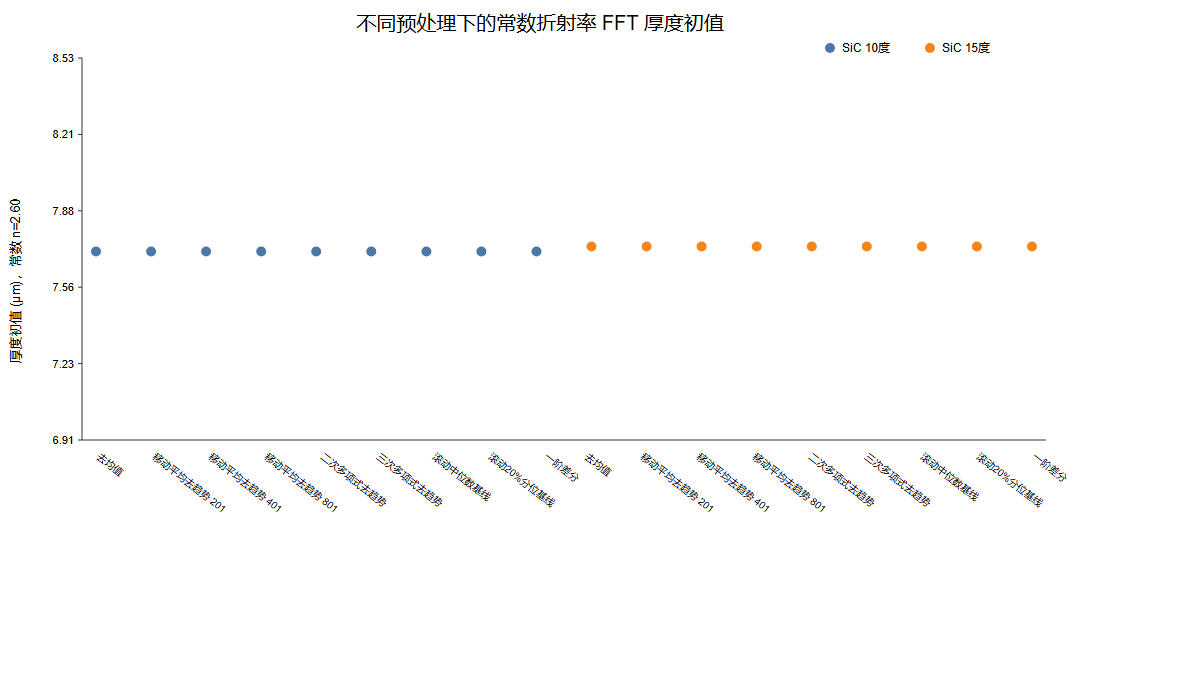
\includegraphics[width=.88\linewidth]{data_processing_fft_thickness_seed.png}
\caption{不同预处理下 FFT 厚度初值。主周期的一致性支持条纹尺度稳定；初值的差异同时表明有效折射率口径不可被忽略。}
\label{fig:fft-cn}
\end{figure}

\section{全谱物理模型与联合求解}
\subsection{Airy/TMM 正演与介电函数约束}
FOD 只使用极值位置，而全谱反演还必须解释振幅和界面多次反射。对于空气--外延层--衬底结构，$r^q_{01}$ 是空气/外延层的直接反射，$r^q_{12}\exp(2{\rm i}\delta)$ 是一次往返后从外延层/衬底界面返回的振幅；其后各次往返再依次乘以 $r^q_{01}r^q_{12}\exp(2{\rm i}\delta)$。将这一等比振幅级数求和，得到 Airy/TMM 形式\cite{Troparevsky2010}：
\begin{equation}
r^q=\frac{r^q_{01}+r^q_{12}\exp(2{\rm i}\delta)}
{1+r^q_{01}r^q_{12}\exp(2{\rm i}\delta)},\quad
\delta=\frac{2\pi}{10^4}\tilde n_1(\nu)d\cos\theta_1\,\nu,
\end{equation}
\begin{equation}
R_{\rm model}=\frac{|r^s|^2+|r^p|^2}{2}.
\label{eq:tmm-cn}
\end{equation}
该模型将厚度、界面 Fresnel 反射、吸收和色散放在同一个正演关系中。

复折射率由 Dong 等人给出的 4H--SiC Lorentz--Drude 介电函数获得\cite{Dong2012}。式中第一项描述 TO--LO 声子响应，第二项为自由载流子 Drude 修正；由介电函数开平方后才得到进入相位与 Fresnel 系数的复折射率：
\begin{equation}
\varepsilon(\nu)=\varepsilon_\infty\left[
\frac{\nu_L^2-\nu^2-{\rm i}\Gamma_L\nu}
{\nu_T^2-\nu^2-{\rm i}\Gamma_T\nu}
-\frac{\nu_p^2}{\nu(\nu+{\rm i}\gamma)}
\right],\qquad \tilde n(\nu)=\sqrt{\varepsilon(\nu)}.
\label{eq:dong-cn}
\end{equation}
式 \eqref{eq:dong-cn} 的声子与 Drude 项来自文献；将其用于本数据、为外延层和衬底分别设置缩放、并加入约束，则是本研究的建模选择。尤其 $\nu_p$ 与载流子浓度相关，故 $s_{\nu_p,\rm epi}\in[0.75,1.75]$、$s_{\nu_p,\rm sub}\in[0.75,1.25]$ 被作为物理边界，而非任意降误差的自由度。

\subsection{共享厚度、变量投影与候选盆地搜索}
对每个入射角，仿射系数由上述线性子问题求解；对厚度和介电参数，采用候选盆地、坐标搜索、受约束局部细化的顺序。先以每个角度的平方残差求和，再以样本数归一化，并加入材料越界惩罚 $\Omega(\eta)$，可写成剖面目标
\begin{equation}
\mathcal L(d,\eta)=
\frac{1}{\sum_aN_a}\sum_a
\min_{\alpha_a,b_a}\sum_i
\left[y_{a,i}-\alpha_aR_a(\nu_i;d,\eta)-b_a\right]^2+\Omega(\eta).
\label{eq:profile-cn}
\end{equation}
这不是把所有参数交给黑箱优化，而是将仪器尺度项显式剖面化、将物理参数限制在可解释范围内，并强制两个角度共享同一 $d$。FFT/FOD 只提供搜索起点；最终由式 \eqref{eq:profile-cn} 下不同候选盆地的可比较损失决定。

\paragraph{全谱拟合结果与模型收益。}
在 Dong2012 表 2 的介电状态下，单角度 TMM 分别在 $7.460\,\um$（$10^\circ$）和 $7.400\,\um$（$15^\circ$）附近取得最优。二者已比 FOD 的角度分离更集中，说明复折射率和多光束干涉解释了部分基线模型无法解释的谱形信息。以该区域为初值，加入共享厚度、仿射剖面化和 $\nu_p$ 物理边界后，局部细化得到 $d^*=7.465\,\um$、联合 RMSE $0.00171152$，相对初始坐标搜索的 $d=7.455\,\um$、RMSE $0.00173772$ 改善 1.508\%。这一改善幅度并不被夸大为外部准确度；它只说明在同一受约束目标下，联合解的内部拟合更好。

\section{反演流程与结果}
中心化、移动平均、低阶多项式、滚动基线和一阶差分等预处理均给出约 $250\,\wn$ 的主周期；滑窗 FFT 范围为 $244.537$--$256.000\,\wn$。因此条纹并非某一平滑参数的伪影。另一方面，常数折射率 FOD 在 $10^\circ$ 和 $15^\circ$ 下分别给出 $7.191\pm0.148\,\um$ 与 $6.603\pm0.089\,\um$，色散 Larruquert FOD 又给出 $5.779\pm0.117\,\um$ 与 $5.292\pm0.065\,\um$。这些差异说明相位证据稳定，但简单模型不足以独立定标厚度。

在 Dong 型介电状态下，单角度搜索先定位到 $7.460\,\um$（$10^\circ$）与 $7.400\,\um$（$15^\circ$）附近。引入共享厚度、仿射剖面化和材料边界后，代表性局部解为 $d^*=7.465\,\um$，联合 RMSE 为 0.00171152；相比初始坐标搜索的 $7.455\,\um$、RMSE 0.00173772，改善为 1.508\%。两角度的独立最优值并不完全一致，因此共享值应被理解为受约束折中，而非两次完全闭合的测量。

\begin{figure}[H]\centering
\begin{minipage}{.48\linewidth}\centering
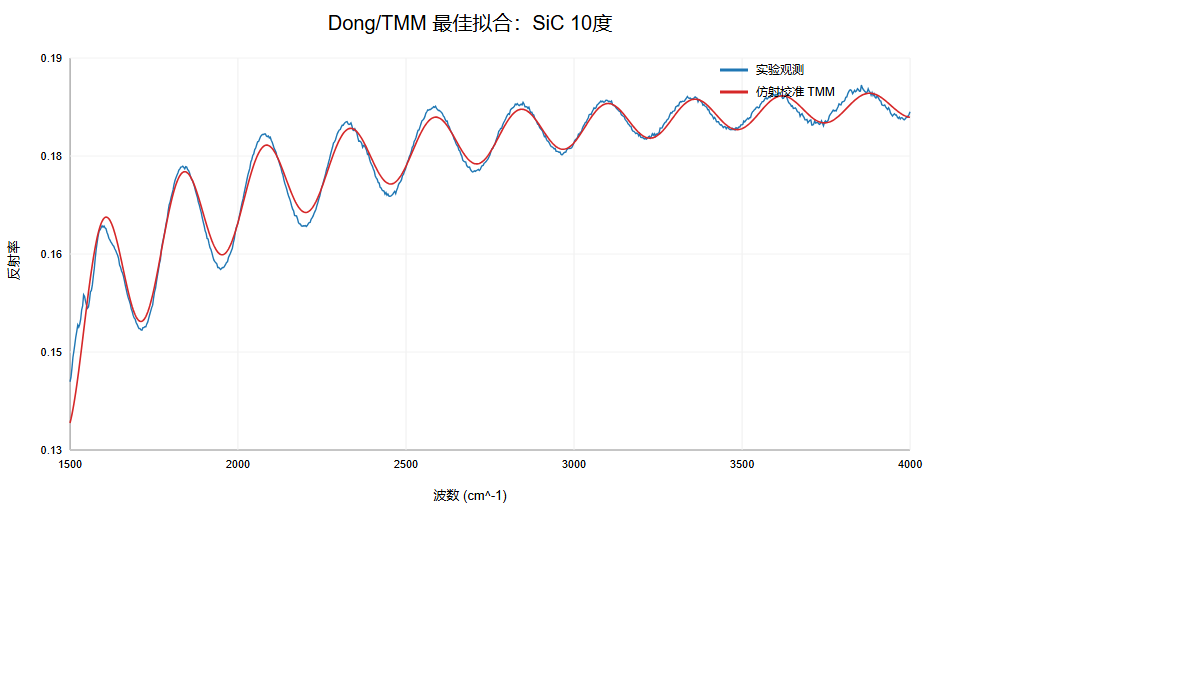
\includegraphics[width=\linewidth]{paper_fig05_tmm_bestfit_SiC_10deg.png}\\[-1mm]\small (a) $10^\circ$
\end{minipage}\hfill
\begin{minipage}{.48\linewidth}\centering
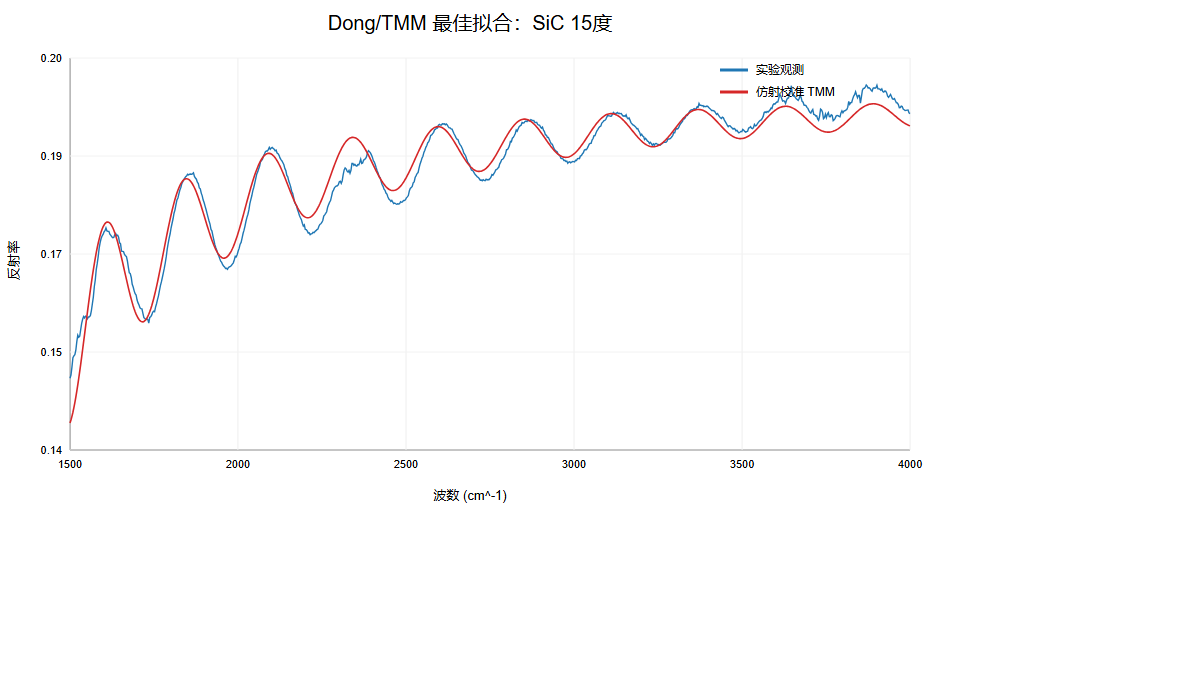
\includegraphics[width=\linewidth]{paper_fig05_tmm_bestfit_SiC_15deg.png}\\[-1mm]\small (b) $15^\circ$
\end{minipage}
\caption{受约束 Dong/TMM 代表点下的双角度拟合。该图检验共享厚度对两次测量的解释能力，必须结合图 \ref{fig:residual-cn} 的残差结构共同阅读。}
\label{fig:tmmfit-cn}
\end{figure}

\begin{table}[H]\centering\small
\caption{厚度结论的证据层级。}
\begin{tabular}{p{.34\linewidth}p{.25\linewidth}p{.30\linewidth}}\toprule
证据 & 记录结果 & 可支持的解释\\\midrule
多路线 FFT & 主周期约 $250\,\wn$ & 存在稳定干涉相位尺度\\
双角度受约束 TMM & $d^*=7.465\,\um$ & 给定模型下的代表值\\
四种频带权重 & $7.465$--$7.485\,\um$ & 局部谷值不由单一权重决定\\
固定材料剖面/自助法 & $7.435$--$7.475\,\um$ 支持区间 & 条件性局部稳定，非总不确定度\\
残差审计 & 15$^\circ$ 残差更大且相关 & 物理解释尚不完备\\\bottomrule
\end{tabular}
\end{table}

等权、FFT 选频、FFT 降权和连续权重下的最小点分别为 $7.465$、$7.485$、$7.475$ 与 $7.470\,\um$，最大移动仅 $0.020\,\um$。固定材料状态下，5\% 剖面支持区间为 $7.435$--$7.475\,\um$；120 次移动分块残差自助法的 2.5\%--97.5\% 分位数为 $7.44488$--$7.46512\,\um$。这些检验说明局部谷值对已记录残差和权重扰动具有稳定性，但没有传播折射率、角度、模型形式和材料先验的不确定性。

\subsection{参数、频带与残差的交叉审计}
为了检查 $7.4$--$7.6\,\um$ 谷值不是单一材料设定的偶然产物，项目分别扫描了 $\nu_p$、$\gamma$、声子阻尼和分析波段。Dong/TMM 的 $\nu_p$ 敏感性给出 $7.440$--$7.580\,\um$，$\gamma$ 敏感性给出 $7.440$--$7.460\,\um$，声子阻尼敏感性给出 $7.400$--$7.480\,\um$。这些结果不构成独立真值，却在不同材料扰动下共同保留同一厚度区域。

对具有不同信息质量的频带，先从等权均方根 $\sqrt{\sum_i e_i^2/N}$ 出发，其中 $e_i=y_i-\hat y_i(d)$。若第 $i$ 个波数点只应贡献相对权重 $w_i$，便以 $\sum_iw_i$ 替代样本数、以 $w_ie_i^2$ 替代单点平方残差，得到加权目标函数
\begin{equation}
J_w(d)=\sqrt{\frac{\sum_iw_i[y_i-\hat y_i(d)]^2}{\sum_iw_i}},\qquad w_i\geq0,
\label{eq:weighted-cn}
\end{equation}
其中 $w_i\equiv1$ 时退化为普通 RMSE。该式为本研究推导的诊断目标，不是为了寻找“最好看的”厚度，而是检验降低可疑波段影响后低谷是否移动。四种权重仅产生 $0.020\,\um$ 的最大位移，因而支持局部结论并非由单一异常频带支撑。

\begin{figure}[H]\centering
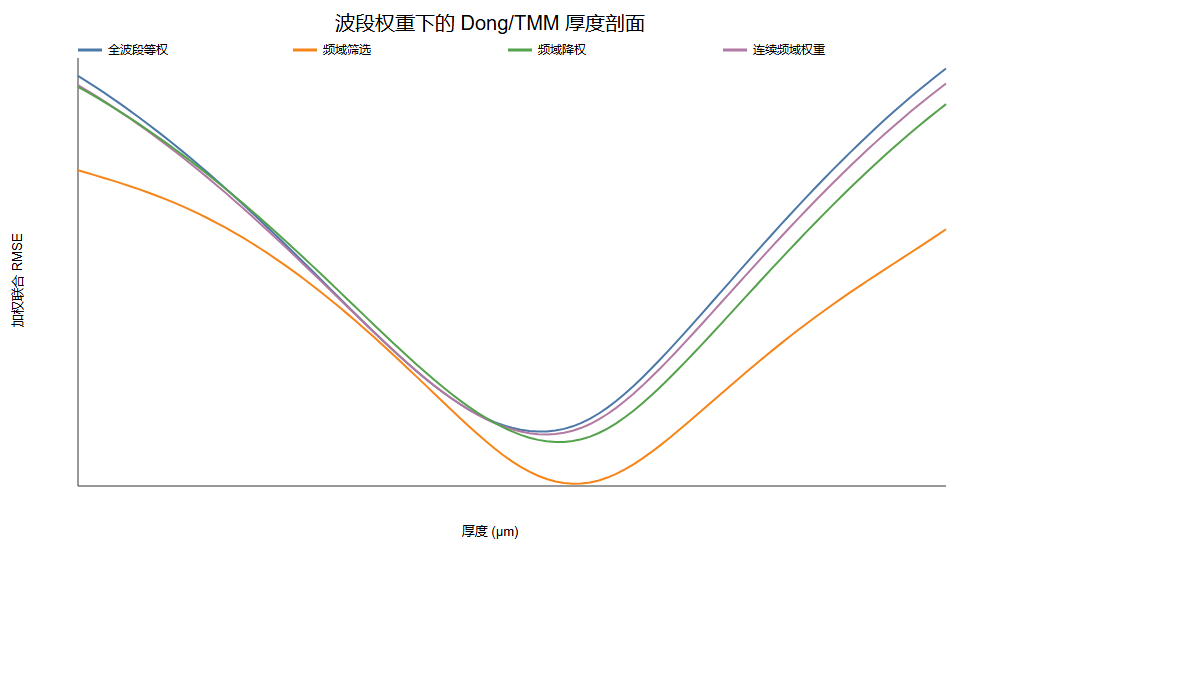
\includegraphics[width=.84\linewidth]{band_weighted_tmm_profile.png}
\caption{四种频带权重下的厚度剖面。低谷位置接近，说明候选厚度不依赖单一频带；该图不是完整物理置信区间。}
\label{fig:weights-cn}
\end{figure}

\begin{figure}[H]\centering
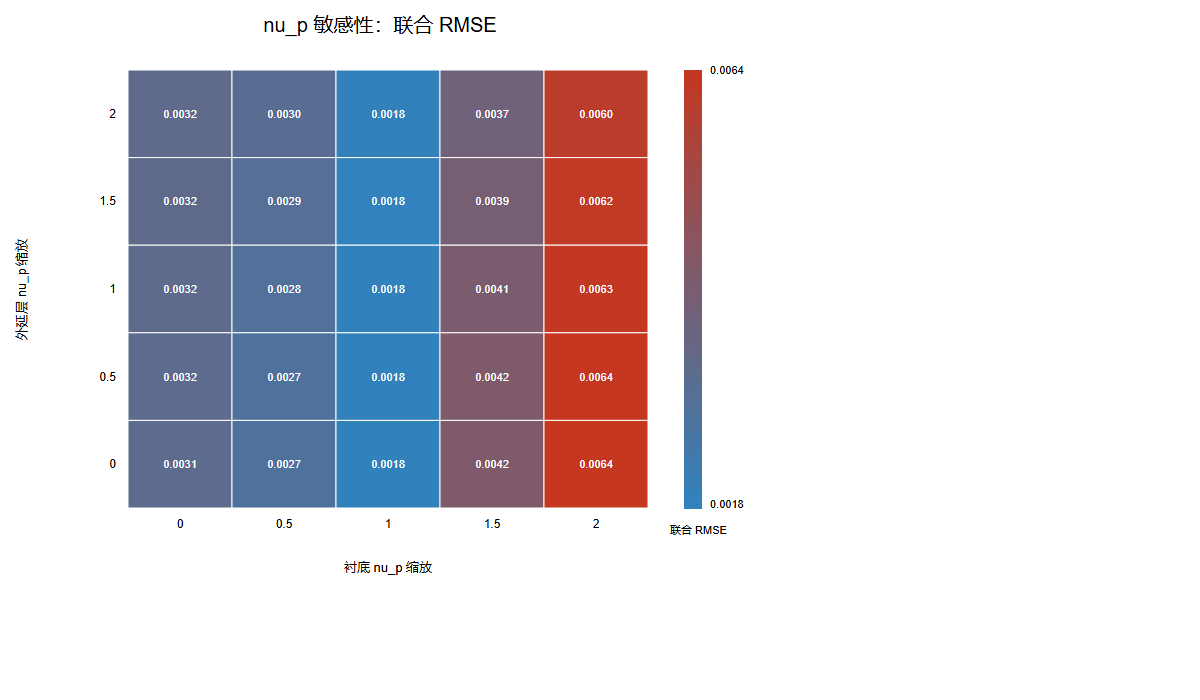
\includegraphics[width=.82\linewidth]{paper_fig10_rmse_heatmap_nu_p_sensitivity.png}
\caption{$\nu_p$ 缩放下的联合 RMSE 热力图。它显示厚度盆地在材料扰动下的延续性，也显示材料参数不确定性仍需纳入结论边界。}
\label{fig:nup-cn}
\end{figure}

\subsection{剖面、分块自助法与模型判别指标}
仅报告最小 RMSE 会掩盖两个问题：低谷是否足够尖锐，以及相邻波数残差是否可以被当作独立噪声。首先，在固定材料状态下扫描 $d=7.200$--$7.700\,\um$，步长为 $0.005\,\um$，5\% RMSE 支持区间为 $7.435$--$7.475\,\um$。这说明在当前材料设定下厚度局部可辨识；它不说明材料设定本身已经被数据唯一确定。

其次，采用长度为 40 个采样点的移动分块残差自助法，进行 120 次重复。其厚度中位数为 $7.455\,\um$，2.5\%--97.5\% 分位数为 $7.44488$--$7.46512\,\um$。使用分块而不是逐点重抽样，是因为反射谱残差在相邻波数处连续相关；这项实验检验的是现有残差结构下局部谷值的重采样稳定性，而不是包含所有物理误差源的置信区间。

\begin{table}[H]\centering\small
\caption{各模型阶段的结果、改进和仍存限制。}
\begin{tabular}{p{.22\linewidth}p{.25\linewidth}p{.23\linewidth}p{.20\linewidth}}\toprule
阶段 & 主要结果 & 相对上一阶段的作用 & 仍存限制\\\midrule
常数 FOD & $7.191/6.603\,\um$ & 多极值回归，弱化单峰误差 & 折射率固定，角度差大\\
色散 FOD & $5.779/5.292\,\um$ & 显式检验色散影响 & 光学常数迁移未闭合\\
FFT/滑窗 FFT & $250\,\wn$；244.537--256.000\,\wn & 独立确认周期尺度 & 不提供唯一物理定标\\
单角度 Dong/TMM & $7.460/7.400\,\um$ & 使用整谱、复折射率与多光束反射 & 两角度仍未完全重合\\
受约束联合 TMM & $7.465\,\um$；RMSE 0.00171152 & 共享厚度并隔离仿射项 & 依赖材料边界\\
权重与重采样审计 & 最大位移 $0.020\,\um$；$7.44488$--$7.46512\,\um$ & 检验局部稳定性 & 只属条件性不确定度\\\bottomrule
\end{tabular}
\end{table}

\section{最终证据一致性审计、结果汇总与模型评价}
\subsection{最终证据一致性审计}
前述稳定性检验分别回答了不同问题，但不能把它们简单并列后即宣布结论。为避免最终判断依赖散落脚本或单次调参，本文只读取已经生成、具有文件记录的实验结果，将其投射到同一厚度轴上；审计不重新调参、不扩大搜索，也不把 FFT/FOD 初值伪装成最终厚度。这样做的目的不是增加“支持性数字”，而是检查独立但有条件的证据是否共同保留同一厚度区域。

图 \ref{fig:finalaudit-cn} 汇总了纳入最终判断的强证据：Dong2012 表 2 状态下的双角度 TMM 分算覆盖 $7.400$--$7.460\,\um$；$\nu_p$ 扰动保留 $7.440$--$7.580\,\um$；$\gamma$、声子阻尼、分析频带、受物理边界约束的局部细化、固定材料剖面、移动分块 bootstrap 和四种权重剖面均未将低谷推出 $7.4$--$7.6\,\um$。因此，最终审计的强证据覆盖为 $7.400$--$7.580\,\um$，而论文采用更易解释且与全部反证一致的 $7.4$--$7.6\,\um$ 作为报告区间。

\begin{figure}[H]\centering
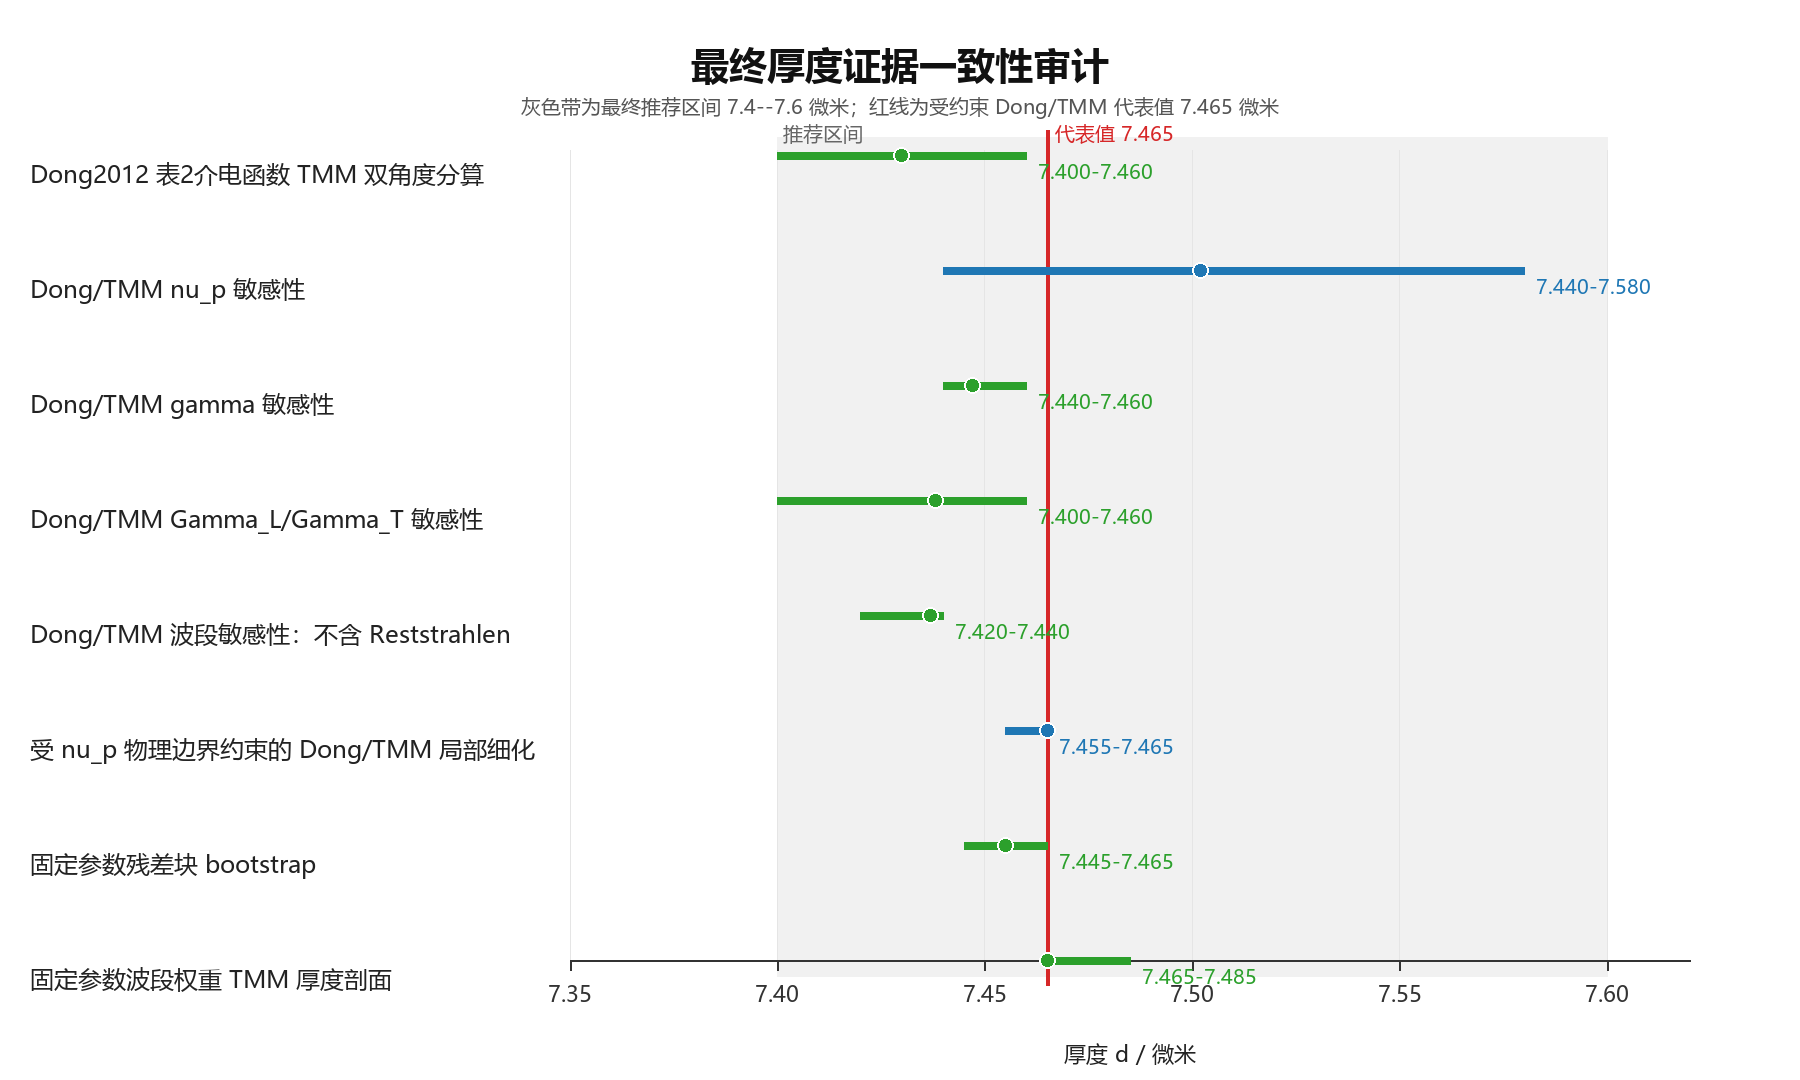
\includegraphics[width=.90\linewidth]{final_evidence_audit.png}
\caption{最终证据一致性审计。每一条带表示一个已记录实验所保留的厚度区域；图中不把 FFT/FOD 初值视作最终厚度证据，也不将这些条件性范围合成为无条件置信区间。}
\label{fig:finalaudit-cn}
\end{figure}

\subsection{结果汇总}
表 \ref{tab:summary-cn} 将研究过程中的关键量、其解释与边界收束在一起。它既保留代表性局部解，也保留不同角度、材料扰动和残差诊断之间未完全闭合的部分；这正是最终报告区间而不是单点认证值的原因。

\begin{table}[H]\centering\small
\caption{关键结果汇总。}\label{tab:summary-cn}
\begin{tabular}{p{.35\linewidth}p{.25\linewidth}p{.29\linewidth}}\toprule
指标 & 记录结果 & 合理解释\\\midrule
全局/滑窗 FFT 周期 & $250\,\wn$；244.537--256.000 $\wn$ & 稳定相位尺度，非唯一厚度标定\\
Dong/TMM 双角度分算 & $7.460/7.400\,\um$ & 全谱模型比 FOD 更集中，但未完全闭合\\
受约束联合代表解 & $7.465\,\um$；RMSE 0.00171152 & 给定模型、边界和权重下的局部代表值\\
$\nu_p$ 敏感性 & $7.440$--$7.580\,\um$ & 材料扰动下的主要厚度盆地\\
固定材料剖面/自助法 & $7.435$--$7.475\,\um$；$7.44488$--$7.46512\,\um$ & 条件性局部稳定，非总不确定度\\
频带权重稳健范围 & $7.465$--$7.485\,\um$ & 低谷不由单一频带或权重决定\\
最终强证据覆盖 & $7.400$--$7.580\,\um$ & 已记录强证据的共同覆盖\\
推荐候选区间 & \textbf{7.4--7.6 $\um$} & 当前最稳妥的测量表述\\\bottomrule
\end{tabular}
\end{table}

\subsection{模型评价与下一步改进}
本研究的优势在于证据顺序清楚：先用多种预处理和滑窗 FFT 确认条纹周期是数据事实，再用 FOD/色散 FOD 显示简化定标的失效边界，最后用双角度 Dong/TMM、变量投影和材料边界进行全谱反演。随后，参数扰动、频带权重、剖面、分块 bootstrap 与残差诊断不再只是附录数字，而是分别检验材料依赖、频带依赖、局部可辨识性、相关残差下的重采样稳定性和模型缺失。

不足也应同时保留：Dong2012 介电参数来自文献样品；$\gamma$ 与声子阻尼的样品特异边界尚未完全建立；外延层 $\nu_p$ 缩放触及上界；且 $15^\circ$ 残差具有结构性。下一阶段优先级不应是继续扩张自由参数，而是补充独立厚度计量、验证入射角和偏振/各向异性，并将材料先验以可追溯方式纳入全局或贝叶斯不确定性传播。

\section{残差、边界与结论}
$10^\circ$ 与 $15^\circ$ 的 RMSE 分别为 0.00131074 和 0.00211230，滞后一阶自相关为 0.9726 和 0.9834。令 $r_j=R_{\rm obs}(\nu_j)-R_{\rm model}(\nu_j)$、$\bar r=m^{-1}\sum_jr_j$；将相邻残差的中心化乘积按总方差归一化，得到一阶自相关
\begin{equation}
\rho_1=\frac{\sum_{j=1}^{m-1}(r_j-\bar r)(r_{j+1}-\bar r)}
{\sum_{j=1}^{m}(r_j-\bar r)^2}
\label{eq:acf-cn}
\end{equation}
计算；当 $\rho_1$ 接近 1 时，残差不是可忽略的独立白噪声。$15^\circ$ 谱在 $1500$--$2500\,\wn$ 与 $3500$--$4000\,\wn$ 区间的失配更持续，且外延层等离子体尺度触及 1.75 上界。残差--频域对齐还显示，这些高残差区与局部条纹证据变化共同出现，因而不能仅通过继续放宽 TMM 参数来处理。这些反证并不否定局部厚度谷值，却明确限制了可作出的主张。

\begin{figure}[H]\centering
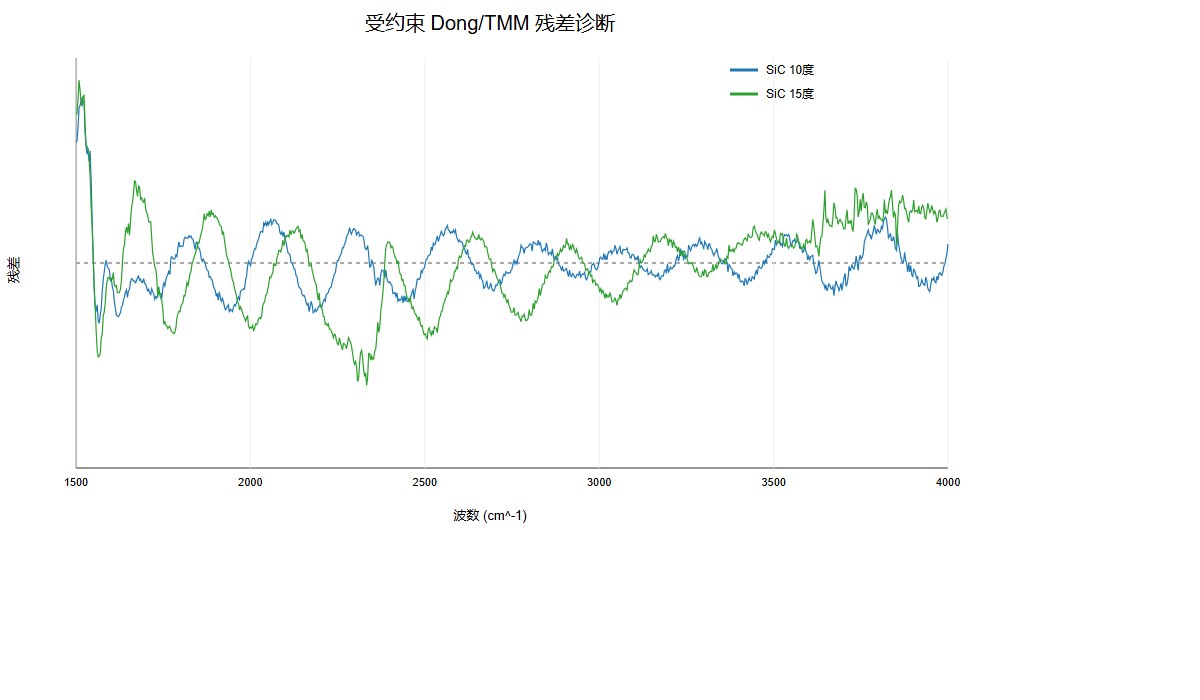
\includegraphics[width=.88\linewidth]{residual_diagnostics_angle_residuals.png}
\caption{双角度残差诊断。尤其是 $15^\circ$ 的结构性残差表明，不能仅以 RMSE 判断模型是否充分解释了测量谱。}
\label{fig:residual-cn}
\end{figure}

因此，本研究最强且最诚实的结论是：现有双角度 FTIR 数据和受约束 TMM 模型支持该 SiC 外延层厚度处于 \textbf{7.4--7.6 \um}，其中 $7.465\,\um$ 是模型条件下的代表值。本文不报告认证厚度、绝对准确度、无条件置信区间或载流子参数测量。下一步应使用独立轮廓仪、截面 SEM 或椭偏仪，并进一步核验入射角、偏振/各向异性和材料先验，以判定 $15^\circ$ 结构性残差的来源。

\section*{数据与代码可用性}
本文使用的原始工作簿、分析脚本与记录结果均保留在项目档案中。分析未引入外部厚度标签或未记录的实验参数。
\section*{参考文献的模型用途说明}
Li 等人的工作\cite{Li2010}提供同类极值级差/FOD 的方法来源，本文据此给出多点相位基线；Dong 等人的工作\cite{Dong2012}提供 4H--SiC Lorentz--Drude 介电函数与 FTIR 反射建模的参数化约束；Troparevsky 等人的工作\cite{Troparevsky2010}提供多层体系 Airy/传输矩阵正演的形式依据。它们支持模型形式与物理约束，不构成本样品厚度的外部真值或准确度验证。
\begin{thebibliography}{9}
\bibitem{Li2010} Z.-Y. Li et al. Methods for Thickness Determination of SiC Homoepilayers by Using Infrared Reflectance Spectroscopy. \emph{Chinese Physics Letters} \textbf{27}, 068103 (2010). doi:10.1088/0256-307x/27/6/068103.
\bibitem{Dong2012} L. Dong et al. Characterization of 4H--SiC substrates and epilayers by Fourier transform infrared reflectance spectroscopy. \emph{Chinese Physics B} \textbf{21}, 047802 (2012). doi:10.1088/1674-1056/21/4/047802.
\bibitem{Troparevsky2010} M. C. Troparevsky, A. S. Sabau, A. R. Lupini and Z. Zhang. Transfer-matrix formalism for the calculation of optical response in multilayer systems: from coherent to incoherent interference. \emph{Optics Express} \textbf{18}, 24715 (2010). doi:10.1364/oe.18.024715.
\end{thebibliography}
\end{document}
